%%%%%%%%%%%%%%%%%%%%%%%%%%%%%%%%%%%%%%%%%%%%%%%%%%%%%%%%%%%%%%%%%%%%%%%%%%%%%%%%
%2345678901234567890123456789012345678901234567890123456789012345678901234567890
%        1         2         3         4         5         6         7         8

%\documentclass[letterpaper, 11 pt, conference]{ieeeconf}  % Comment this line out
                                                          % if you need a4paper
\documentclass[a4paper, 11pt, conference]{ieeeconf}      % Use this line for a4
                                                          % paper

\IEEEoverridecommandlockouts                              % This command is only
                                                          % needed if you want to
                                                          % use the \thanks command
\overrideIEEEmargins
% See the \addtolength command later in the file to balance the column lengths
% on the last page of the document



% The following packages can be found on http:\\www.ctan.org
%\usepackage{graphics} % for pdf, bitmapped graphics files
%\usepackage{epsfig} % for postscript graphics files
%\usepackage{mathptmx} % assumes new font selection scheme installed
%\usepackage{times} % assumes new font selection scheme installed
%\usepackage{amsmath} % assumes amsmath package installed
%\usepackage{amssymb}  % assumes amsmath package installed
\usepackage{authblk}
\title{\LARGE \bf
PDRAM - Page Replacement policy for Heterogeneous Memory architectures
}
\usepackage{graphicx}
\usepackage{float}
\author{Bharadwaj Krishnamurthy}
\author{Prashanth Balasubramanian}
\author{Choungki Song}
\affil{Department of Electrical Engineering \\University of Wisconsin-Madison}


\begin{document}



\maketitle
\thispagestyle{empty}
\pagestyle{empty}


%%%%%%%%%%%%%%%%%%%%%%%%%%%%%%%%%%%%%%%%%%%%%%%%%%%%%%%%%%%%%%%%%%%%%%%%%%%%%%%%
\begin{abstract}

Operating Systems offer Inter Process Communication (IPC) mechanisms for sharing data among processes. This work is aimed at studying latency and throughput of three such IPC techniques - Pipes, TCP/IP Sockets and Shared memory. To evaluate the accuracy of the timing measurements, different timing APIs were studied and the one with least variance and high resolution was chosen for the experiments. IPC mechanisms are evaluated against varying message packet lengths. Shared memory technique was able to achieve a throughput of the order of 10 GB/S for message length of 512KB. Sockets however offer better single message latency compared to other techniques. 
\end{abstract}

\vspace{3mm}
\begin{keywords}
inter-process communication, pipes, sockets, shared memory buffer, timing measurement, ipc benchmarking
\end{keywords}
\vspace{5mm}
%%%%%%%%%%%%%%%%%%%%%%%%%%%%%%%%%%%%%%%%%%%%%%%%%%%%%%%%%%%%%%%%%%%%%%%%%%%%%%%%


\section{INTRODUCTION}

\vspace{3mm}
	The memory requirements of modern applications have been increasing.  However, DRAM capacity has not been able to keep up with the memory requirements of applications due to slow increase in DRAM density.  The low DRAM capacity results in data residing in DRAM to be swapped out to persistent storage when the memory is scarce, thereby causing frequent page faults.  This causes a lot of traffic between memory and disk, and decrease system performance.
Until now, system architects have tackled this problem by using multiple DIMMs per channel and multiple channels. However, it results in increased maintenance cost because the DRAM consumes static power due to refresh operation.  The static power increases as the capacity increases.  Therefore, the current approach in untenable. 

	Non-volatile RAM technologies such as Phase Change RAM (PCRAM) have much higher densities compared to DRAM.  Non-volatile memory does not consume static power as amount as DRAM consumes, and the cost per capacity is cheaper than that of DRAM.  Besides, recent PCRAM technology improves latency dramatically. Although NVRAM technologies are still slower compared to DRAM, the advantages have forced its adoption as an alternative to DRAMs  into the physical address space  However, PCRAM also has a critical drawback.  Its write latency of PCRAM is one or two order slower than that of DRAM.  In addition, it has a limitation on the number of write operations. Both DRAM and PCRAM have their own pros and cons. One could combine the pros of DRAM and PCRAM to form contiguous memory space and present a larger physical memory to OS for it run applications.

	The hybrid memory architecture poses difficulties in form of latency mismatches between PCRAM and DRAM, write wearing in PCRAM and different read and write latencies in PCRAM. The latency mismatch cannot be avoided by increasing the writes to DRAM as it would wear off the memory. Thus, deciding which pages are to be mapped to PCRAM and the ones to be retained in DRAM and dynamic movement of pages would impact the performance of such architectures. This work aims at identifying variables which would impact the paging policy and borrow concepts from Hot page policy \cite{meswani2015heterogeneous} to device a suitable mechanism.

\section{RELATED WORK} \vspace{2mm}
\subsection{Cached DRAM} \vspace{1mm}
	In \cite{qureshi2009scalable}, a approach for hybrid memory is proposed to use DRAM as a cache for PCRAM acting as a main memory.  Write operation from the processor is cached in the DRAM to improve write wear leveling of PCRAM. And all the read operation is processed with DRAM.  Although it uses a hybrid memory architecture, the DRAM is transparent to system software as if there are only PCRAMs and the DRAM caching is entirely managed in hardware. This involves a lot of hardware design effort to support this architecture. First, DRAM controller does not know where data is, which makes the memory access latency unpredictable. Seconds, DRAM needs periodic refresh and during refresh all the memory accesses stalls even if PCRAM does not need periodic refresh. Third, this architecture increases memory access latency due to sequential operations: tag read and compare, and then reading data at different timing depending on the his/miss. We plan to use PCRAM as part of the physical address space being entirely managed by the system software.

\subsection{Page movement policy} \vspace{1mm}
\textit{\textbf{Hot page policy}}

	A recent paper introduces hybrid memory using HBM and DRAM \cite{meswani2015heterogeneous} to mitigate the bandwidth limitation of DRAM with the use of high bandwidth memory.  The authors introduce hot page policy, that the frequently accessed pages will be moved into HBM from DRAM, with tracking page access counts which is incremented by each access and initialized to 0 at each epoch. The policies used would be a great starting point for our project. In addition, we need to keep in mind the asymmetry between read and write latencies and the lower endurance of the PCRAM in making page migration decisions.

\textit{\textbf{LRU page policy}}
	The use of mixed DRAM with PCRAM is proposed as a hybrid memory \cite{seok2011migration}.  Dynamic  page monitoring and migration between the PRAM and DRAM is done based on access pattern.  If there is a write operation in the page is promoted into DRAM queue and one of the read queue is swapped out.  To mitigate write wearing, all the write transaction is monitored while it causes another write operation due to page swapping operation. Their policy aims to improve the write endurance of PCRAM and hence keep write-bound pages on the DRAM and read-bound pages on the PRAM. As we explained in introduction section, the latency of PCRAM is worse than that of DRAM, so using DRAM in most cases helps to improve performance if there is no memory pressure.  Our goal is to improve the read and write latencies while keeping write endurance in mind. Hence, we need a more sophisticated policy than the one followed.

\textit{\textbf{Dynamic page migration}}
PDRAM\cite{dhiman2009pdram} employs Dynamic page management using counters to distribute write operation through entire PCRAM.  The PCRAM is marked in one of the three state: free, used-free - which is - but not reached a specified threshold, and threshold-free that the page is accessed over the limit.  The threshold-free page is marked as a not-available until all the pages in PCRAM are marked threshold-free.  Once all the page are marked threshold-free, the page is marked a free page, which makes variation of capacity over time. However, they use only two memory allocation policies agnostic of the write and read capabilities to the page. We plan to implement a more write/read aware allocation policy.

\textit{\textbf{Miscellaneous policy in the kernel}}
The paper \cite{mogul2009operating} proposes several page allocation heuristics that need to be kept in mind while writing system software for hybrid memory: page type, file type, file reference modes, application-supplied page attributes, page history.  Although these heuristics are primarily proposed for Flash devices to improve their endurance, we could borrow some of these ideas to fine-tune our page migration policy.


\section{DESIGN} \vspace{2mm}

We take a two pronged approach in managing physical pages in DRAM and the PCRAM. First, we decide on placement of pages at allocation time. An optimal choice will help reduce the amount of migration back and forth between DRAM and PCRAM. Secondly, we regularly look at physical pages in the DRAM and PRAM and decide to migrate the pages based on their activity. We discuss the two approaches in more detail in the following subsections.

\subsection{Heterogeneous architecture} \vspace{1mm}
Different memories can be used as main memories even though there is no real system which uses this methodology while many people are working on this part to provide enough environment. 

\vspace{2mm}
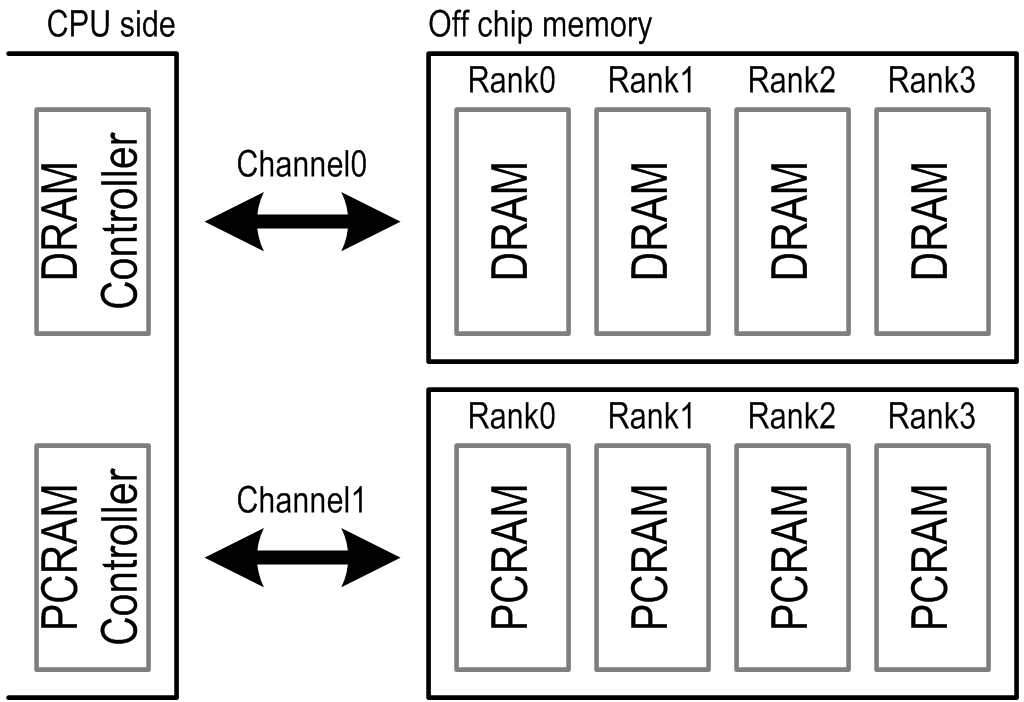
\includegraphics[width=0.45\textwidth]{Architecture/1-HeteroMem.jpg}
\begin{center}
  {\textsc{Figure.1 Memory channels and ranks}}
\end{center}

Those memories needs different memory controller to read and write data because the latency of access and access procedures are quite different each other as depicted in figure.1. 

In addition to this, we should take address mapping into account.  Normally, OS does not care about address mapping which usually controlled by hardware setting \cite{kaseridis2011minimalist}.  Most common address mapping is to parallelize multiple channels of memory to utilize the memory efficiently as in figure.3 (a). By the way, we should change the address mapping because each memories are on different channels on our work. For example, in typical mapping 4K byte of page is spread out into channels which means there is no method which move page data into DRAM from PCRAM.  Therefore our work assume that DRAM and PCRAM use different memory controller and the channel address is allocated as a MSB in address mapping.

\vspace{3mm}

\includegraphics[width=0.45\textwidth]{Architecture/2-OldAddrMap.jpg}
\begin{center}
  {\textsc{(a) Typical Mapping}}
\end{center}

\vspace{3mm}
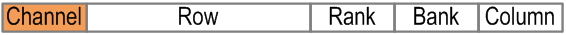
\includegraphics[width=0.45\textwidth]{Architecture/3-NewAddrMap.jpg}
\begin{center}
  {\textsc{(b) Proposed Mapping}}
\end{center}
\begin{center}
  {\textsc{Figure.2 Address Mapping}}
\end{center}

\subsection{Page Allocation Policy} \vspace{1mm}
Previous work on linux kernel support for phase change memory [Linux kernel] takes a similar approach while allocating pages. During page allocation of user mode pages, we modify the kernel allocation to satisfy requests to code, text and shared library pages in the PCRAM. We do this for two main reasons. First, code and text pages are read only by construction. By allocating such pages in the PCRAM, we do not incur the costs of significantly high write latencies. Second, executable pages in modern systems are generally cached in dedicated hardware instruction caches . In most architectures, the thrashing is restricted only to the lower level caches. Hence, the amount of instruction misses (and, thereby the memory accesses) is relatively lower compared to the data cache counterparts. As a result, the amount of memory accesses are significantly less. We decided to incur the extra cost of higher read latency in the PCRAM for such pages in the hope that such an increase would be amortized over time. We present the evaluation this policy in Section <Evaluation>.

\subsection{Page Migration policies} \vspace{1mm}
It is often insufficient  to distinguish between DRAM and PCRAM only at allocation time. Resident pages vary in characteristics even during the course of a program. For example, a CPU bound workload might do a few memory accesses followed by a  compute intensive task. On traditional systems, such pages are marked inactive and are swapped out of disk when there is memory pressure.  In such cases, it would be best to offload such pages to a slower and denser memory (PCRAM). We implement two different policies to implement migration.

\vspace{1mm}

\textit{\textbf{Proactive Migration}}
As the name suggests, we constantly monitor the resident pages in the DRAM and proactively migrate them from DRAM to PCRAM. In this endeavour, we divide the system execution time into epochs. At the end of every epoch, we selectively migrate the inactive pages. This selection is based on the characteristics of physical pages. A summary of our decision is shown in <Table>. The advantage of this approach is that memory pressure is seldom created in the DRAM. However, this may result in memory pressure in the PCRAM. Although in practice one could have a higher capacity PCRAM for the same cost as a DRAM and alleviate this issue, we do consider this in our policy and migrate the active pages in the PCRAM back to DRAM. This also addresses the problem of pages that are being frequently accessed bearing the extra latency costs. The downside of this approach is that the policy may migrate pages when there is no actual memory pressure resulting in energy and migration latency costs.

\textit{\textbf{Lazy Migration}}:
In this approach, we migrate pages lazily. Instead of constantly migrating pages every epoch, we migrate the pages only when there is memory pressure in the DRAM. The migration happens before kswapd daemon kicks in to swap out the inactive pages. This way, we still avoid the time-costly kswapd daemon but at the same time keep the memory pressure in the DRAM low. The downside of this approach is that the migration might inadvertently cause the kswapd to wake up in the PCRAM which results in page swapping anyway.

\subsection{Page movement overhead} \vspace{1mm}
In order to move page from PCRAM to DRAM, the operation should be separated as followed: 1. Activate a wordline in PCRAM and DRAM respectively, 2. Read a page from PCRAM, 3. Write the page into DRAM, 4. Precharge the each wordlines. The unit size for read and write access is 64Byte, therefore 64 read accesses from PCRAM and 64 write accesses to DRAM are required to move 4KB page. The Figure.3 is the our timing diagram for page move.  The active latency, read latency, precharge latency in PCRAM are 55.5ns, 14ns, 14ns each other, while those in DRAM are 14ns, 14ns and 15ns each other \cite{lee2009architecting}\cite{miconddr4}. The latency for a page movement is a summation of active latency of PCRAM, read latency, 64 column to column latency (4 clk), read to write latency (about 20 clk), and precharge latency for DRAM.  The total latency at DDR3200, clock cycle is 0.625ns, is about 260ns which is only considered memory latency.  If we consider control latency by DRAM controller or DMA, it may be increased to about 300ns for a page movement.

	The power for a page movement is also considered in terms of active operation in both, precharge operation in both, and read operation in PCRAM and write operation in DRAM from previous work \cite{lee2009architecting}.  The wordline size in a channel, which consists of 8 chips, is 8KB which affects active and precharge power.  A page size is 4KB which affects the power for read and write access.  The equation for total power consumption for a page movement is expressed as 
AP@PCRAM + AP@DRAM + PP@PCRAM + PP@DRAM + RP@PCRAM + WP@DRAM,
where AP stands for active power, PP for precharge power, RP for read power, and WP for write power.  The total power for page movement is about 300nJ.

\section{EVALUATION} \vspace{2mm}

\subsection{Experimental Setup}
The proposed design was implemented on linux-4.5 kernel. The modified kernel was booted on a qemu emulator with ubuntu rootfs. Qemu emulated a system with x86\_64 cpu and 1024MB of RAM. Qemu emulator was executed on a host system with 4098 MB of DRAM and quad-core i5 CPU. Host and emulated system configurations are summarized in \ref{host_machine} and \ref{vm_machine} respectively. "enable-kvm" option enabled Qemu to use processor extensions for virtualization and to speed up the execution. For simpler policy implementation huge transparent pages were turned off. Ubuntu 12.04 was used as root file system and the choice of rootfs was solely based on the ease of setting up network interfaces and standard packages through apt-get interface.

\vspace{1mm}

\begin{table}[H]
\def\arraystretch{1.5}
\caption{Experiment setup - Host System}
\label{host_machine}
\begin{center}
\begin{tabular}{|p{2.5cm}||p{4cm}|}
\hline
Architecture & x86\_64\\[0.75ex]
\hline
CPU & Intel(R) Core(TM) i5-4570 \\ [0.75ex]
\hline
No. of cores & 4 \\ [0.75ex]
\hline
CPU Frequency& 3192.899 MHz \\ [0.75ex]
\hline
Cache & 6144 KB \\ [0.75ex]
\hline
Total memory & 4096 MB \\ [0.75ex]
\hline
Linux Version &2.6.32\-573.7.1.el6.x86\_64 \\ [0.75ex]
\hline
\end{tabular}
\end{center}
\end{table}

\begin{table}[H]
\def\arraystretch{1.5}
\caption{Experiment setup - Emulated System}
\label{vm_machine}
\begin{center}
\begin{tabular}{|p{3cm}||p{3.5cm}|}
\hline
Architecture & x86\_64\\[0.75ex]
\hline
No. of cores & 1 \\ [0.75ex]
\hline
L1 I-Cache & 32 KB \\ [0.75ex]
\hline
L1 D-Cache & 32 KB \\ [0.75ex]
\hline
L2 Cache & 4096 KB \\ [0.75ex]
\hline
Total memory & 1024 MB \\ [0.75ex]
\hline
DRAM memory & 512 MB \\ [0.75ex]
\hline
PCRAM memory & 512 MB \\ [0.75ex]
\hline
Linux Version & 4.5 \\ [0.75ex]
\hline
Fake NUMA Nodes & 2 \\ [0.75ex]
\hline
\end{tabular}
\end{center}
\end{table}

\vspace{1mm}

The PCRAM node was emulated using the fake numa option in the linux kernel. This option enabled us to split the available memory into two equal halves. Node 0 was considered as DRAM and node 1 was PRAM. \textit{numactl} provided user level knobs that bound the memory allocation to the desired node. We employed this to restrict program execution to DRAM node in baseline model. Many other tools like \textit{numastat},\textit{vmstat} and \textit{zoneinfo} were used to monitor memory allocation and migration at run-time. Apart from the standard packages we have added event monitors in the kernel to get finer details of page migration. These are read using external kernel modules.

\begin{figure*}
 \begin{center}
  	{\textsc{Table III Detail information of Benchmark programs}}
  \end{center}
  \vspace{2mm}
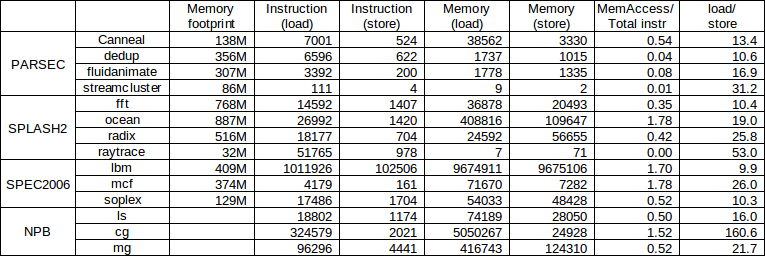
\includegraphics[width=\textwidth]{Architecture/4-BenchPrograms.png}
\end{figure*}

\subsection{Benchmarks}
	Each benchmark suits has memory intensive and cpu intensive workloads. Here, we want to break down which benchmark programs are memory intensive for evaluation.  We selected lbm, mcf and soplex from SPEC2006 based on the evaluation \cite{jaleel2010memory}, and canneal, dedup, fluidanimate and streamcluster from PARSEC \cite{bienia2008parsec}, fft, ocean, radix and raytrace from SPLASH2 \cite{woo1995splash}.
We evaluated each benchmarks program with valgrind tools to obtain information of memory footprint and the number of access on cache and memory.  Table.3 shows the results of it. The memory footprint is measured with massif in valgrind. The instruction and memory is measured with cachegrind in valgrind and the unit in this column is K, which means the value should be multiplied by 1,024ea.  MemAccess/Totalinstr, which unit is percent, is how much instructions cause main memory accesses and load/store is the ratio of load per store instruction. Therefore, we can divide the programs into memory intensive: ocean, lbm, mcf, cg and cpu intensive: fft, dedup, fluidanimate, raytrace, and read-oriented: cg, raytrace, mcf, radix, and write-oriented:dedup, fft, lbm, soplex.

\subsection{PIN trace program}
	We use the pin trace to profile the page table being accessed because there is no method to keep track of the number of pages being accessed in kernel.  At the original pin program, each instructions for memory access are printed into a file with virtual address format. It results in generating big size of file because the instructions are more than 1G.  In order to record the number of page are access and reduce the size of file, first we add some code to translate virtual address to physical address, and second we add a way counting the number of memory access in page and printing page number and its accessed information without printing all the memory accesses to reduce the trace results, lastly we changed counting method only for 2 or 4 partitions for our work.  The reason why we changed is because counting the each page increases the run time dramatically.

\bibliographystyle{plain}
\bibliography{bibliography.bib}

\end{document}
